\section{Model Architecture}
\label{sec:arch}

Our proposed system consists of two components, shown in Figure~\ref{fig:TTSArchitecture}:
\begin{inparaenum}[(1)]
  \item a recurrent sequence-to-sequence feature prediction network with
    attention which predicts a sequence of mel spectrogram frames from an
    input character sequence, and
  \item a modified version of WaveNet which generates time-domain waveform samples
    conditioned on the predicted mel spectrogram frames.
\end{inparaenum}

\subsection{Intermediate Feature Representation}

In this work we choose a low-level acoustic representation: mel-frequency
spectrograms, to bridge the two components. Using a representation
that is easily computed from time-domain waveforms allows us to train the two
components separately. This representation is also smoother than waveform
samples and is easier to train using a squared error loss because it is
invariant to phase within each frame.

A mel-frequency spectrogram is related to the linear-frequency spectrogram, \ie
the short-time Fourier transform (STFT) magnitude. It is obtained by applying a
nonlinear transform to the frequency axis of the STFT, inspired by measured
responses from the human auditory system, and summarizes the frequency content
with fewer dimensions.
%
Using such an auditory frequency scale has the effect of emphasizing details in
lower frequencies, which are critical to speech intelligibility, while
de-emphasizing high frequency details, which are dominated by fricatives and
other noise bursts and generally do not need to be modeled with high fidelity.
%
Because of these properties, features derived from the mel scale have
been used as an underlying representation for speech recognition for
many decades \cite{davis:mel}.

While linear spectrograms discard phase information (and are therefore lossy),
algorithms such as Griffin-Lim \cite{Griffin84signalestimation} are capable of
estimating this discarded information, which enables time-domain conversion
via the inverse short-time Fourier transform. Mel spectrograms discard even more
information, presenting a challenging inverse problem.
%
However, in comparison to the linguistic and acoustic features used in
WaveNet, the mel spectrogram is a simpler, lower-level acoustic
representation of audio signals. It should therefore be straightforward for a
similar WaveNet model conditioned on mel spectrograms to generate audio,
essentially as a neural vocoder.
%
% Furthermore, using 80 frequency buckets to compute a mel spectrogram with a
% frame hop of 12.5~ms, only 80 values were needed to represent each frame as
% compared to the 300 samples in a waveform sampled at 24~kHz, which should make it
% easier to predict.
%
Indeed, we will show that it is possible to generate high quality audio from mel
spectrograms using a modified WaveNet architecture.


\subsection{Spectrogram Prediction Network}
\label{ssec:c2f}

% char2mel params: http://cnsviewer2/cns/jn-d/home/jonathanasdf/brain/rs=6.3/char2mel_169147260/train/params.txt

%\subsubsection{Features}
%task.input.waveform_processor.frame_size_ms : 50.0
%task.input.waveform_processor.frame_step_ms : 12.5
%task.input.waveform_processor.magnitude_floor : 0.01
%task.input.waveform_processor.mel_channels : 80
%task.input.waveform_processor.mel_lower_edge_hertz : 125.0
%task.input.waveform_processor.mel_upper_edge_hertz : 7600.0
% wow: so wavenet extends the bandwidth!!!
%
%NOTE: pre_emphasis is *not* used in WaveformProcessor.LogMelScaleFilterbankEnergies.
%task.input.waveform_processor.pre_emphasis : 0.97
As in Tacotron, mel spectrograms are computed
through a short-time Fourier transform (STFT) using a 50~ms frame size, 12.5~ms
frame hop, and a Hann window function. We experimented with a 5~ms frame hop to
match the frequency of the conditioning inputs in the original WaveNet, but
the corresponding increase in temporal resolution resulted in significantly more
pronunciation issues.

% TODO(ronw): Is the below true and do we need to note it?
% Note that we do not use preemphasis.
%
We transform the STFT magnitude to the mel scale using an 80 channel
mel filterbank spanning 125~Hz to 7.6~kHz, followed by log dynamic
range compression.
%
Prior to log compression, the filterbank output magnitudes are clipped to a
minimum value of 0.01 in order to limit dynamic range in the logarithmic domain.

% \subsubsection{Encoder}
%task.encoder.emb_dim : 512
The network is composed of an encoder and a decoder with attention.
The encoder converts a character sequence into a hidden
feature representation which the decoder consumes to predict a
spectrogram.
%
Input characters are represented using a learned 512-dimensional character
embedding, which are passed through
%task.encoder.conv_dropout_prob : 0.5
%task.encoder.conv_layers : 3
%task.encoder.conv_tpl.activation : 'RELU'
%task.encoder.conv_tpl.batch_norm : True
%conv_p.filter_shape = [5, 1, p.emb_dim, p.emb_dim]
a stack of 3 convolutional layers each containing 512 filters with shape
$5\times1$, \ie where each filter spans 5 characters, followed by batch
normalization \cite{ioffe2015batch} and ReLU activations.
%
As in Tacotron, these convolutional layers model longer-term
context (\eg $N$-grams) in the input character sequence.
%task.encoder.num_lstm_layers : 1
%task.encoder.lstm_cell_size : 256
%task.encoder.lstm_tpl.zo_prob : 0.1
%
The output of the final convolutional layer is passed into a single
bi-directional \cite{Schuster:1997:BRN:2198065.2205129} LSTM
\cite{Hochreiter:1997:LSM:1246443.1246450} layer containing 512 units
(256 in each direction) to generate the encoded features.

% \subsubsection{Attention}
The encoder output is consumed by an attention network which
summarizes the full encoded sequence as a fixed-length context vector
for each decoder output step.
%
We use the location-sensitive attention from
\cite{chorowski2015attention}, which extends the additive attention
mechanism \cite{bahdanau2014neural} to use cumulative attention
weights from previous decoder time steps as an additional feature.
This encourages the model to move forward consistently through the
input, mitigating potential failure modes where some
subsequences are repeated or ignored by the decoder.
%
%task.decoder.attention.hidden_dim : 128
%task.decoder.attention.location_filter_size : 31
%task.decoder.attention.location_num_filters : 32
Attention probabilities are computed after projecting inputs % TODO: does this need an equation
and location features to 128-dimensional hidden representations.
Location features are computed using 32 1-D convolution filters of
length 31.

% \subsubsection{Decoder}
The decoder is an autoregressive recurrent neural network which
predicts a mel spectrogram from the encoded input sequence one
frame at a time.
%
%task.decoder.target_pre_net.activation : 'RELU'
%task.decoder.target_pre_net.batch_norm : False
%task.decoder.target_pre_net.dropout_prob : 0.5
%task.decoder.target_pre_net.hidden_layer_dims : [256, 256]
The prediction from the previous time step is first passed through a
small \emph{pre-net} containing 2 fully connected layers of 256 hidden ReLU units.
We found that the pre-net acting as an information bottleneck was essential for
learning attention.
%
%task.decoder.rnn_layers : 2
%task.decoder.rnn_cell_dim : 1024
%task.decoder.rnn_cell_tpl.zo_prob : 0.1
The pre-net output and attention context vector are concatenated and
passed through a stack of 2 uni-directional LSTM layers with 1024 units.
%
The concatenation of the LSTM output and the attention context vector is
projected through a linear transform to predict the target
spectrogram frame.
%task.decoder.post_edit_convnet_filter_shapes : [[5, 1, None, 512], [5, 1, 512, 512], [5, 1, 512, 512], [5, 1, 512, 512], [5, 1, 512, None]]
Finally, the predicted mel spectrogram is passed through a 5-layer convolutional
\emph{post-net} which predicts a residual to add to the prediction to improve the
overall reconstruction.
%
Each post-net layer is comprised of 512 filters with shape $5\times1$ with
batch normalization, followed by $\tanh$ activations on all but the final layer.

We minimize the summed mean squared error (MSE) from before and after the
post-net to aid convergence.  We also experimented with a log-likelihood loss by
modeling the output distribution with a Mixture Density Network
\cite{Bishop94mixturedensity,Schuster99onsupervised} to avoid assuming
a constant variance over time, but found that these were more difficult to
train and they did not lead to better sounding samples.

%->eos prediction
% https://cs.corp.google.com/piper///depot/google3/learning/brain/research/babelfish/tts/decoder.py?l=226
In parallel to spectrogram frame prediction, the concatenation of
decoder LSTM output and the attention context
is projected down to a scalar and passed through a sigmoid activation
to predict the probability that the output sequence has completed.
This ``stop token'' prediction is used during inference to allow the model to
dynamically determine when to terminate generation instead of always generating
for a fixed duration.
Specifically, generation completes at the first frame for which this probability
exceeds a threshold of 0.5.

The convolutional layers in the network are regularized using dropout
\cite{srivastava2014dropout} with probability 0.5, and LSTM layers are
regularized using zoneout \cite{krueger2016zoneout} with probability 0.1. In
order to introduce output variation at inference time, dropout with probability
0.5 is applied only to layers in the pre-net of the autoregressive decoder.

In contrast to the original Tacotron, our model uses simpler
building blocks, using vanilla LSTM and convolutional layers in
the encoder and decoder instead of ``CBHG'' stacks and GRU recurrent
layers.
%
We do not use a ``reduction factor'', \ie each decoder step
corresponds to a single spectrogram frame.


\begin{figure}[t!]
\centering
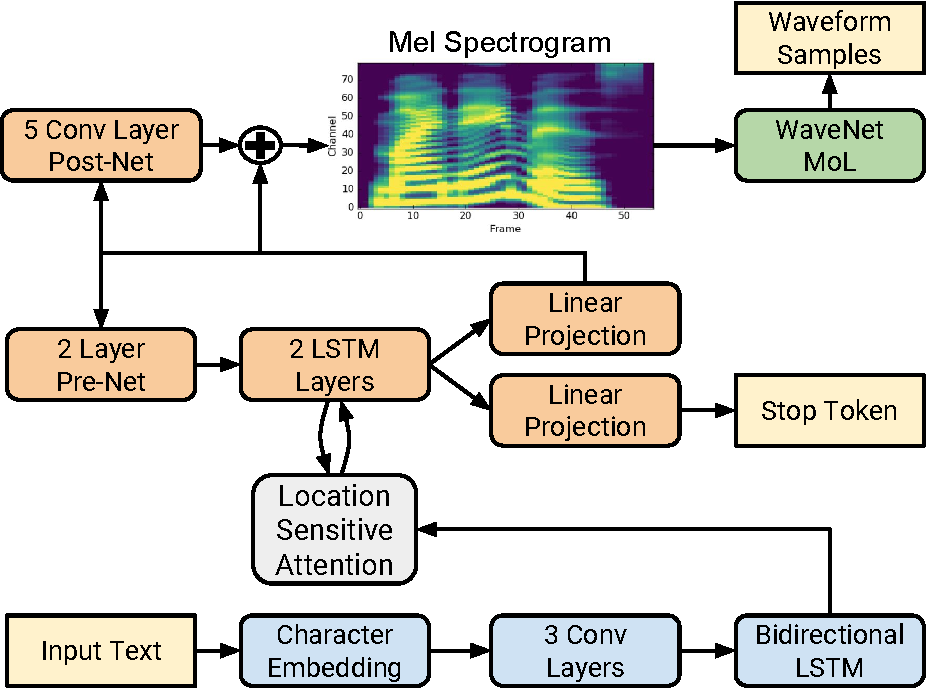
\includegraphics[width=0.98\columnwidth]{TTSArchitecture.pdf}
\caption{Block diagram of the Tacotron 2 system architecture.}
\label{fig:TTSArchitecture}
\end{figure}


\subsection{WaveNet Vocoder}
\label{ssec:wavenet}

We use a modified version of the WaveNet architecture from \cite{45774} to
invert the mel spectrogram feature representation into time-domain waveform
samples.
%
As in the original architecture, there are 30 dilated convolution layers,
grouped into 3 dilation cycles, \ie the dilation rate of layer k
($k=0\ldots 29$) is $2^{k\pmod{10}}$.
%
To work with the 12.5~ms frame hop of the spectrogram frames, only 2 upsampling
layers are used in the conditioning stack instead of 3 layers.

Instead of predicting discretized buckets with a softmax layer,
we follow PixelCNN++ \cite{DBLP:journals/corr/SalimansKCK17} and
Parallel WaveNet \cite{FasterWaveNet} and use a 10-component
mixture of logistic distributions (MoL) to generate 16-bit samples at 24~kHz.
%
To compute the logistic mixture distribution, the WaveNet stack output is passed
through a ReLU activation followed by a linear projection to predict
parameters (mean, log scale, mixture weight) for each mixture component.
%
The loss is computed as the negative log-likelihood of the ground truth sample.
